\documentclass{article}
\usepackage{graphicx} % Required for inserting images
\usepackage[russian]{babel}


\title{Теорема Пифагора}
\author{Автор}
\date{19.09.2025}


\begin{document}
\maketitle
\tableofcontents
\newpage



\section{Введение}
Теорема Пифагора — одна из важнейших теорем евклидовой геометрии. Она находит применение в самых разных областях:
\begin{itemize}
    \item геометрия и тригонометрия
    \item физика
    \item инженерные расчёты
    \item компьютерная графика
\end{itemize}



\section{Формулировка теоремы}
\textbf{Слова:} В прямоугольном треугольнике квадрат гипотенузы равен сумме квадратов катетов.
\begin{equation}
    c^2 = a^2 + b^2
\end{equation}
Как видно из формулы 1, знание двух сторон позволяет найти третью.



\section{Доказательство (набросок)}
\begin{flushleft}
Одно из доказательств основывается на площади квадрата, составленного
из четырёх одинаковых прямоугольных треугольников и малого квадрата
в центре. Раскладывая площадь двумя способами, получаем $c^2 = a^2 + b^2$.
\end{flushleft}



\section{Примеры расчёта}
\textbf{Пример 1}
\[
a = 3, \ \ b = 4
\]
\[
c = \sqrt{a^2+b^2}=\sqrt{9+16}=5
\]
\textbf{Пример 2}
\begin{enumerate}
    \item Дано: a = 5, \ \ b = 12
    \item Решение:
\end{enumerate}
\[
c = \sqrt{5^2+12^2}=\sqrt{25+144}=13
\]



\section{Таблица значений}
\begin{center}
\begin{tabular}{|c|c|c|}
\hline
Катет a & Катет b & Катет c \\
\hline
3 & 4 & 5\\
\hline
5 & 12 & 13\\
\hline
7 & 24 & 25\\
\hline
\end{tabular}
\end{center}



\section{Иллюстрация}
Ниже пример изображения:
\begin{center}
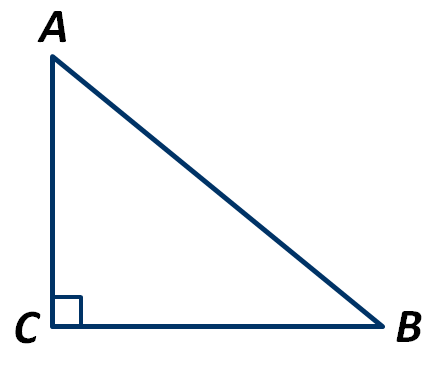
\includegraphics[width=0.5\textwidth]{triangle.png}
\end{center}



\section{Заключение}
Теорема Пифагора — один из краеугольных камней геометрии, помогающий решать
множество практических задач.



\section{Ссылки и литература}
\begin{itemize}
    \item Википедия: Теорема Пифагора
    \item Классические учебники геометрии
\end{itemize}



\end{document}